\documentclass[UTF8,a4paper,10pt]{ctexart}
\usepackage[left=2.50cm, right=2.50cm, top=2.50cm, bottom=2.50cm]{geometry}
%页边距
\CTEXsetup[format={\Large\bfseries}]{section} %设置章标题居左

%%%%%%%%%%%%%%%%%%%%%%%
% -- text font --
% compile using Xelatex
%%%%%%%%%%%%%%%%%%%%%%%
% -- 中文字体 --
%\setmainfont{Microsoft YaHei}  % 微软雅黑
%\setmainfont{YouYuan}  % 幼圆    
%\setmainfont{NSimSun}  % 新宋体
%\setmainfont{KaiTi}    % 楷体
%\setmainfont{SimSun}   % 宋体
%\setmainfont{SimHei}   % 黑体
% -- 英文字体 --
%\usepackage{times}
%\usepackage{mathpazo}
%\usepackage{fourier}
%\usepackage{charter}

%\usepackage{helvet}

\usepackage{amsmath, amsfonts, amssymb} % math equations, symbols
\usepackage[english]{babel}
\usepackage{color}	% color content
\usepackage{graphicx}	% import figures
\usepackage{url}	% hyperlinks
\usepackage{bm} 	% bold type for equations
\usepackage{multirow}
\usepackage{booktabs}
\usepackage{epstopdf}
\usepackage{epsfig}
\usepackage{algorithm}
\usepackage{algorithmic}
\usepackage{listings}
\usepackage{xcolor}
\usepackage{booktabs}
\usepackage{zhnumber}
\usepackage{longtable}
\usepackage{subfigure}
\usepackage{float}
\usepackage{caption}
\usepackage{subfigure}
\renewcommand\thesection{\zhnum{section}}
\renewcommand \thesubsection {\arabic{section}}
\renewcommand{\algorithmicrequire}{ \textbf{Input:}}
% use Input in the format of Algorithm  
\renewcommand{\algorithmicensure}{ \textbf{Initialize:}}
% use Initialize in the format of Algorithm  
\renewcommand{\algorithmicreturn}{ \textbf{Output:}}
% use Output in the format of Algorithm  
%%%%%%%%%%%%%%%%%%
\usepackage{listings}
\usepackage{color}
\definecolor{dkgreen}{rgb}{0,0.6,0}
\definecolor{gray}{rgb}{0.5,0.5,0.5}
\definecolor{mauve}{rgb}{0.58,0,0.82}
\lstset{frame=tb,
  language=Python,
  aboveskip=3mm,
  belowskip=3mm,
  showstringspaces=false,
  columns=flexible,
  basicstyle={\small\ttfamily},
  numbers=left,%设置行号位置none不显示行号
  %numberstyle=\tiny\courier, %设置行号大小
  numberstyle=\tiny\color{gray},
  keywordstyle=\color{blue},
  commentstyle=\color{dkgreen},
  stringstyle=\color{mauve},
  breaklines=true,
  breakatwhitespace=true,
  escapeinside=``,%逃逸字符(1左面的键),用于显示中文例如在代码中`中文...`
  tabsize=4,
  extendedchars=false %解决代码跨页时,章节标题,页眉等汉字不显示的问题
}

%%%%%%%%%%%%%%%%%%%%%%%%%%%%
\usepackage{fancyhdr} %设置页眉、页脚
\pagestyle{fancy}
\lhead{}
\chead{}
%\rhead{\includegraphics[width=1.2cm]{fig/ZJU_BLUE.eps}}
\lfoot{}
\cfoot{}
\rfoot{}
\fancyfoot[RE,RO]{~\thepage~}

\fancyhead[RE,RO]{计算物理导论 \quad 2022春季学期 \quad 作业12 \quad 何翼成}

%%%%%%%%%%%%%%%%%%%%%%%
%  设置水印
%%%%%%%%%%%%%%%%%%%%%%%
%\usepackage{draftwatermark}         % 所有页加水印
%\usepackage[firstpage]{draftwatermark} % 只有第一页加水印
% \SetWatermarkText{Water-Mark}           % 设置水印内容
% \SetWatermarkText{\includegraphics{fig/ZJDX-WaterMark.eps}}         % 设置水印logo
% \SetWatermarkLightness{0.9}             % 设置水印透明度 0-1
% \SetWatermarkScale{1}                   % 设置水印大小 0-1    

\usepackage{hyperref} %bookmarks
\hypersetup{colorlinks, bookmarks, unicode} %unicode

\title{\textbf{蒙特卡洛方法求解Ising模型}}
\author{ 何翼成 \thanks{学号:520072910043; \newline
    邮箱地址:heyicheng@sjtu. edu. cn} }
\date{\today}

\begin{document}
\maketitle

%\begin{abstract}
%这是一篇中文小论文。这个部分用来写摘要。摘要的章标题默认是英文,还没找到改成中文的方法:(
%\end{abstract}
\section*{Project 1}
\section{题目分析}
%%%以下为插入图片模板
%\quad \newline
	\begin{figure}[!htbp]
		\centering
		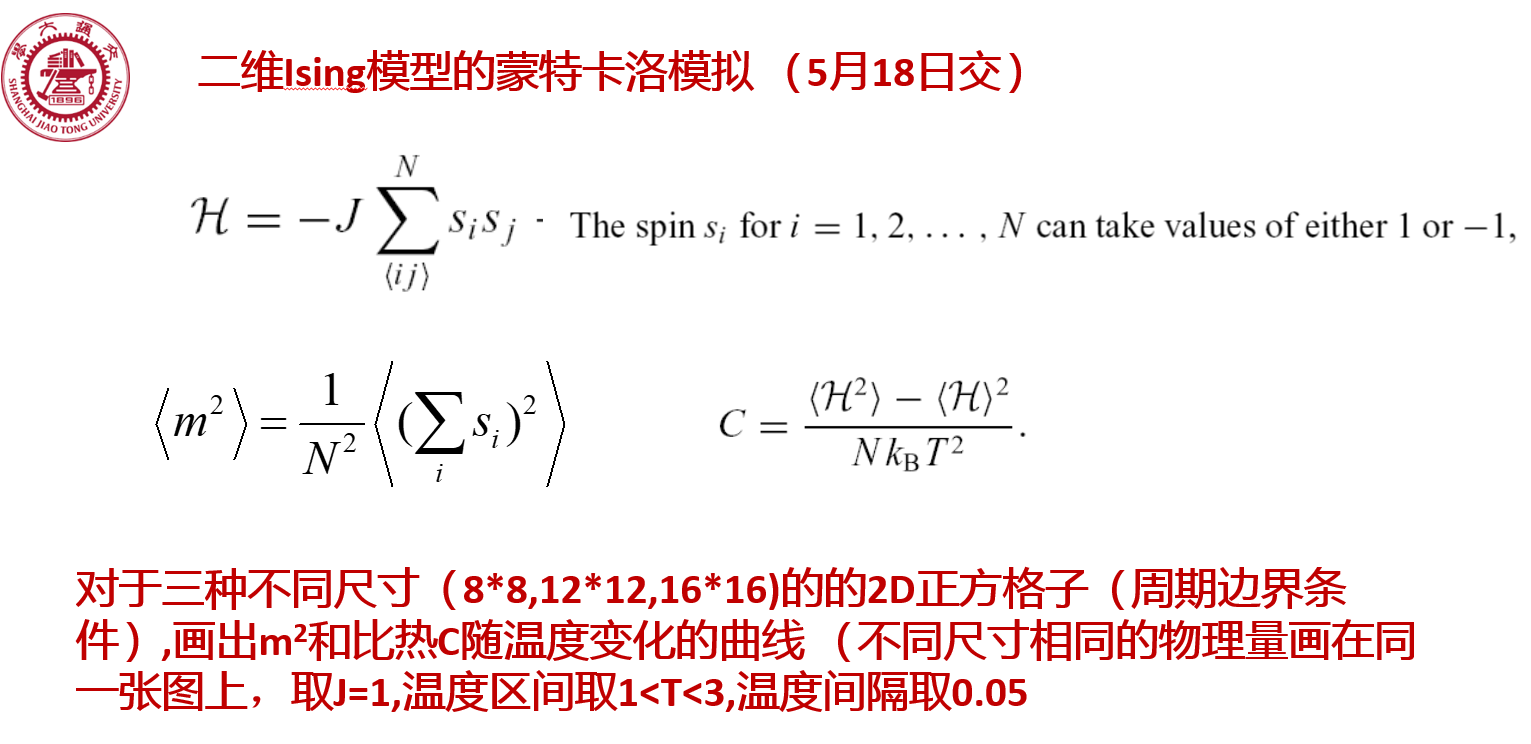
\includegraphics[width=1\textwidth,height=0.6\textwidth]{pictures/pro.png}
		\caption{题目总览} \label{project1}
	\end{figure}



\section{代码展示}
\lstset{language=matlab}
\begin{lstlisting}
    clear;clc;
    Ls=[8,12,16];
    dT=0.025;Tspan=1:dT:3;
    
    %生成随机初始条件的自旋矩阵
    N=6e6;%计算次数
    L_m2=zeros(3,length(Tspan));L_C=L_m2;%分配数据位置
    for ii=1:3
        L=Ls(ii);%确认2D正方格子尺寸
        M=randi([0,1],L,L)*2-1;%生成随机磁矩矩阵
        m2_T=zeros(1,length(Tspan));H2_T=m2_T;H1_T=m2_T;%分配数据位置
        for Tn=1:length(Tspan)
            T=Tspan(Tn);
            m2_s=[];H2_s=[];H1_s=[];%分配数据位置
            for nn=1:N
                M_1=M;%保留磁矩矩阵的原信息
                loc=randi([1,L],1,2);%随机翻转自旋的坐标
                x=loc(1);y=loc(2);
                M_2=M;M_2(x,y)=-M_1(x,y);%翻转后的磁矩矩阵
                %计算能量差
                pudM=pud(M);
                deltaE=2*M_1(x,y)*(pudM(x+2,y+1)+pudM(x,y+1)+pudM(x+1,y+2)+pudM(x+1,y));
                %判断状态是否保留
                flag=Metro(deltaE,T);
                if flag==1
                    M=M_2;
                else
                    M=M_1;
                end
                %计算当前时刻的各物理量,保留以进行时间平均
                m2=(sum(M(:))^2)/(L^4);
                H1=H(M);
                H2=H1^2;
                m2_s(end+1)=m2;
                H2_s(end+1)=H2;
                H1_s(end+1)=H1;
            end
            %计算m^2,H^2,H在T=Tspan(Tn)下的期望值
            l=length(m2_s);
            m2_s_avg_Tn=sum(m2_s)/l;
            H2_s_avg_Tn=sum(H2_s)/l;
            H1_s_avg_Tn=sum(H1_s)/l;
            %将上述数值记录在提前分配的内存中,以方便进行下一步计算
            m2_T(Tn)=m2_s_avg_Tn;
            H2_T(Tn)=H2_s_avg_Tn;
            H1_T(Tn)=H1_s_avg_Tn;
            disp("任务数为"+ii+"/3,已完成第"+Tn+"轮计算,进度为"+Tn/length(Tspan)*100+"%")
        end
        L_m2(ii,:)=m2_T;
        L_C(ii,:)=(H2_T-H1_T.^2)./(L^2*Tspan.^2);
    end
    figure(1)
    plot(Tspan,L_m2(1,:),'r',Tspan,L_m2(2,:),'k',Tspan,L_m2(3,:),'b')
    xlabel('Temperature');ylabel('<m^2>');
    legend("L=8","L=12","L=16");
    figure(2)
    plot(Tspan,L_C(1,:),'r',Tspan,L_C(2,:),'k',Tspan,L_C(3,:),'b')
    xlabel('Temperature');ylabel('C');
    legend("L=8","L=12","L=16");
    %%
    %Metropolis算法函数的定义
    function flag=Metro(deltaE,T)
        beta=1/T;
        if deltaE<=0
            p=1;
        else
            p=exp(-beta*deltaE);
        end
        z=rand();
        if z<p
           flag=1;
        else
            flag=0;
        end
    end
    %%
    %Pud,辅助计算。输出(L+2)**2的矩阵
    function pudM=pud(M)
    L=size(M,1);
    pudM=zeros(L+2,L+2);%分配储存空间
    %pudding,采用周期性边界条件
    pudM(2:(L+1),2:(L+1))=M;
    %行的移动
    pudM(1,2:(L+1))=M(L,:);
    pudM(L+2,2:(L+1))=M(1,:);
    %列的移动
    pudM(2:(L+1),1)=M(:,L);
    pudM(2:(L+1),L+2)=M(:,1);
    end
    
    %能量计算
    function E=H(M)
    L=size(M,1);
    pudM=pud(M);
    H=0;
    for i=2:L
        for j=2:L
            H=H-pudM(i,j)*(pudM(i,j-1)+pudM(i,j+1)+pudM(i-1,j)+pudM(i+1,j));
        end
    end
    E=H/2;
    end
\end{lstlisting}

\section{结果分析与结论}

\begin{figure}[!htbp]
    \centering
    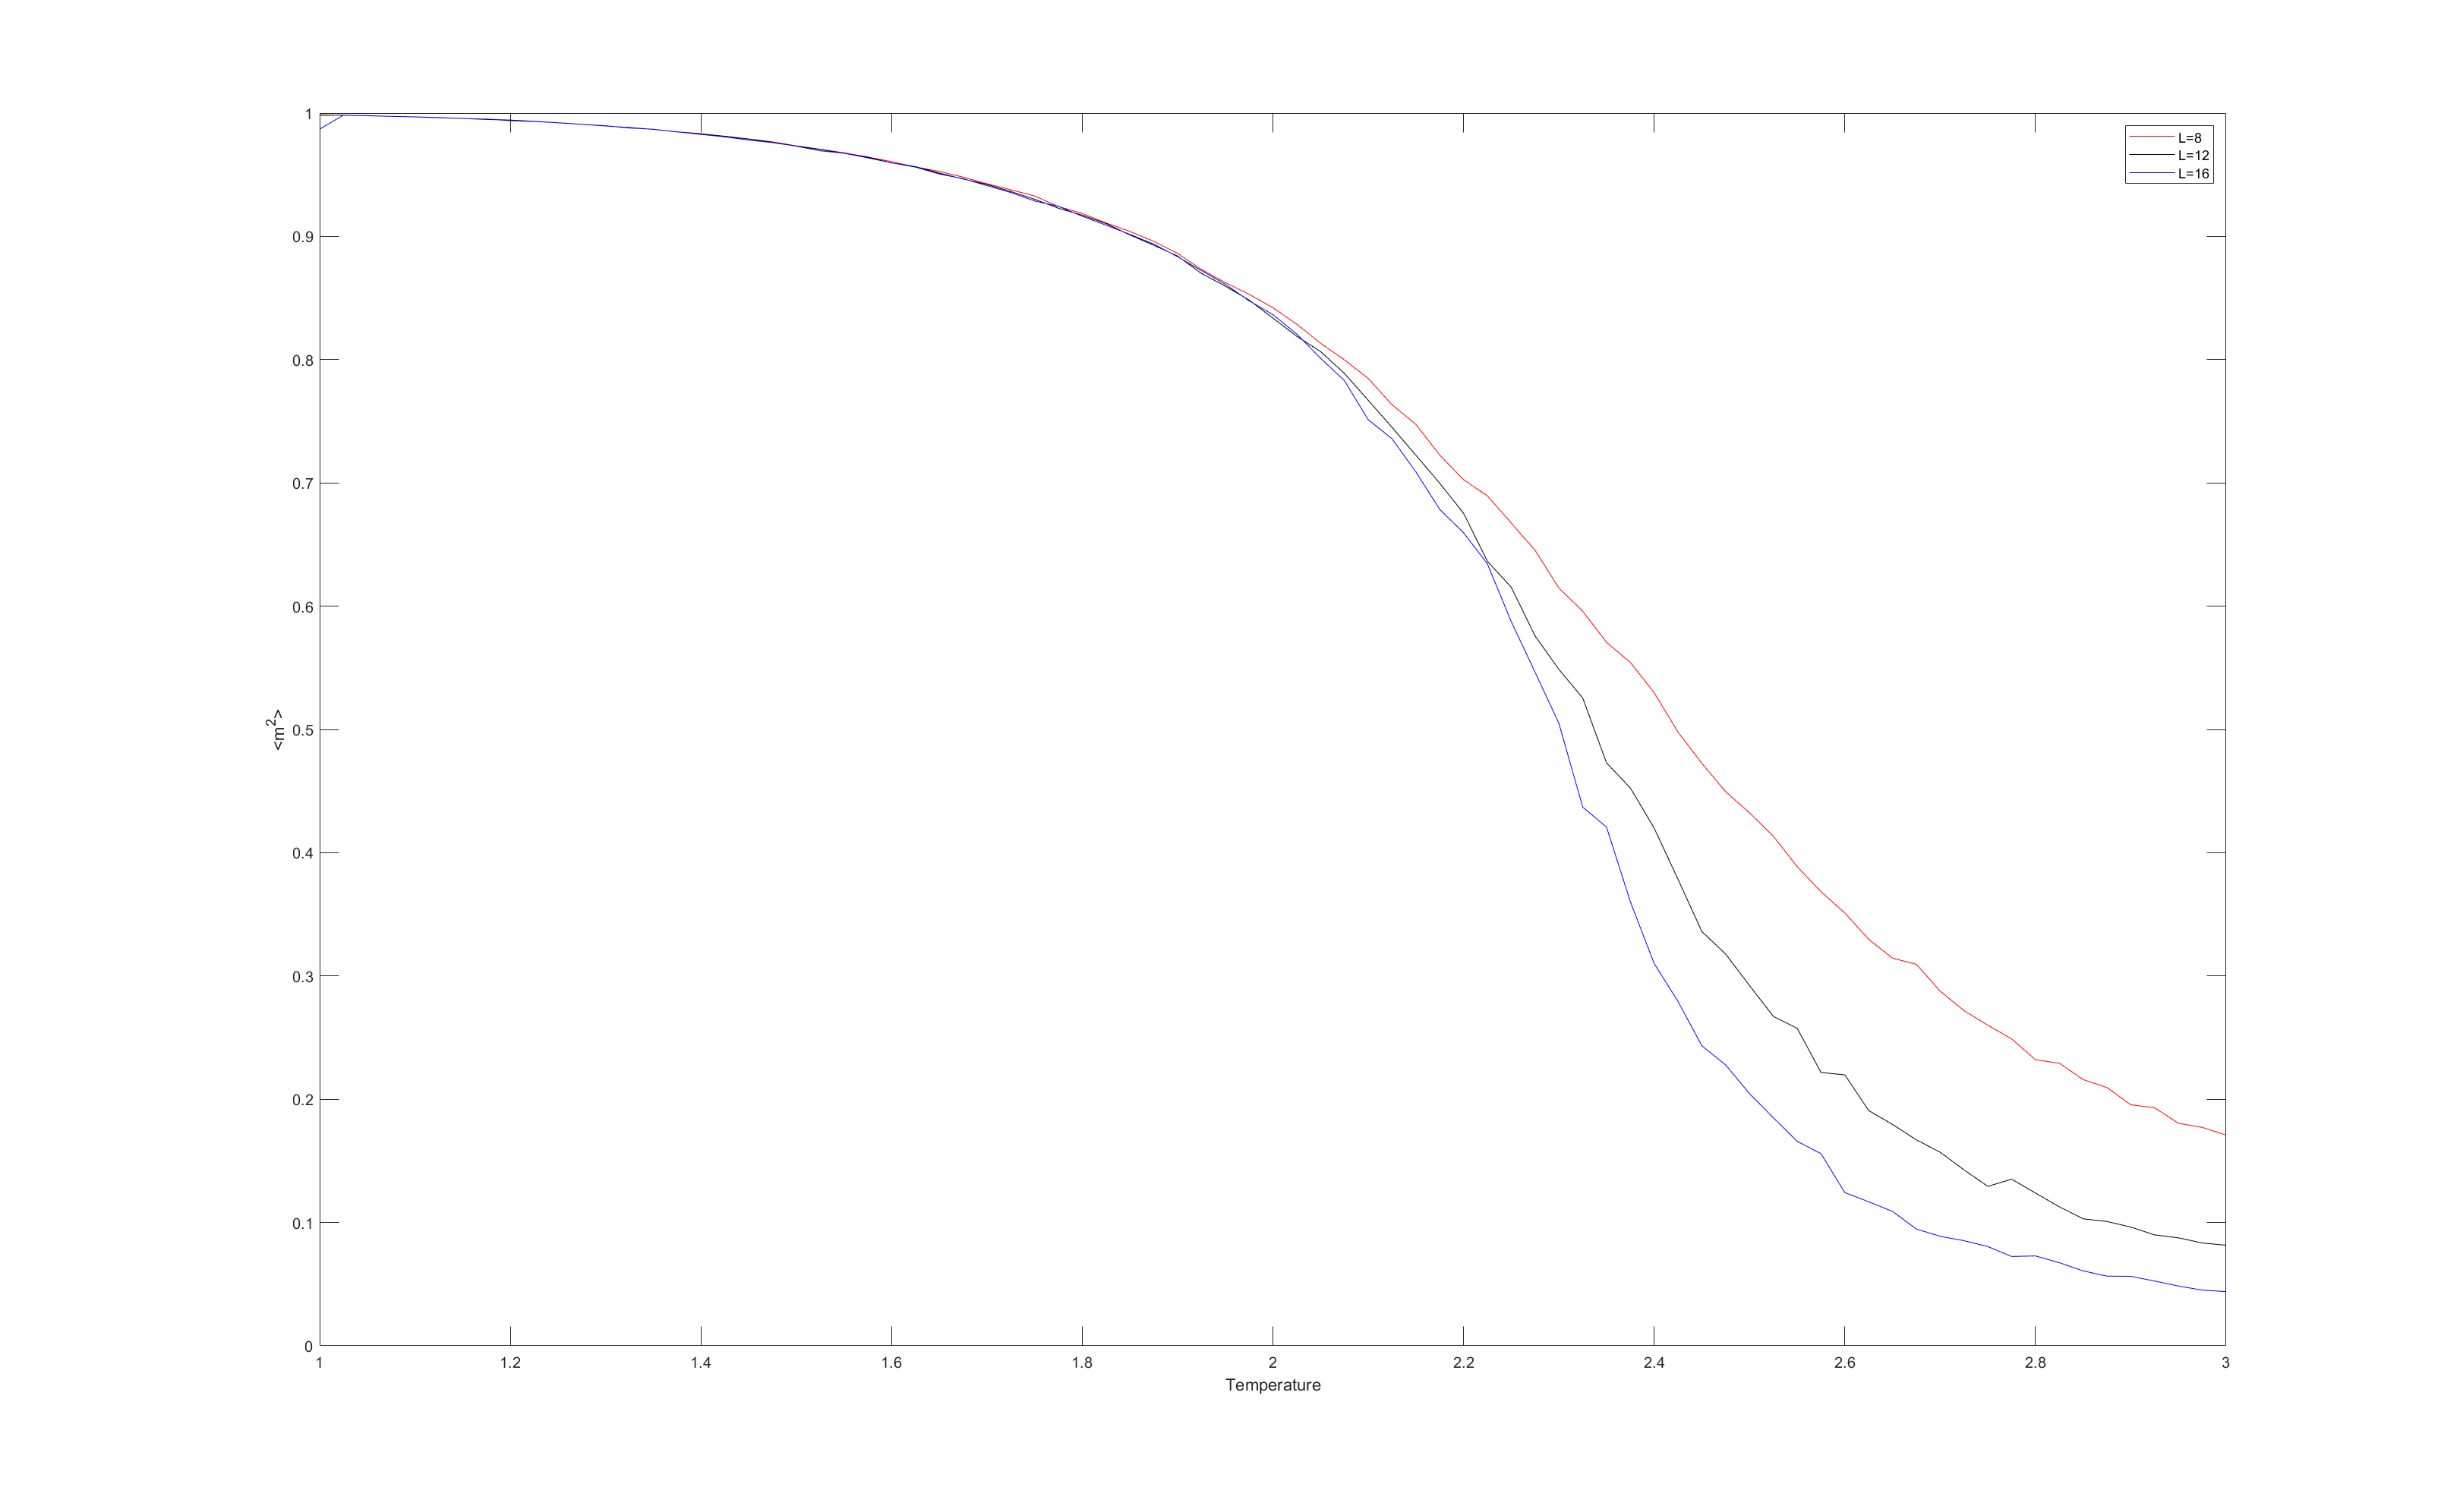
\includegraphics[width=1\textwidth,height=1\textwidth]{pictures/m2.png}
    \caption{m的平方随温度T的变化} \label{m2}
\end{figure}

\begin{figure}[!htbp]
    \centering
    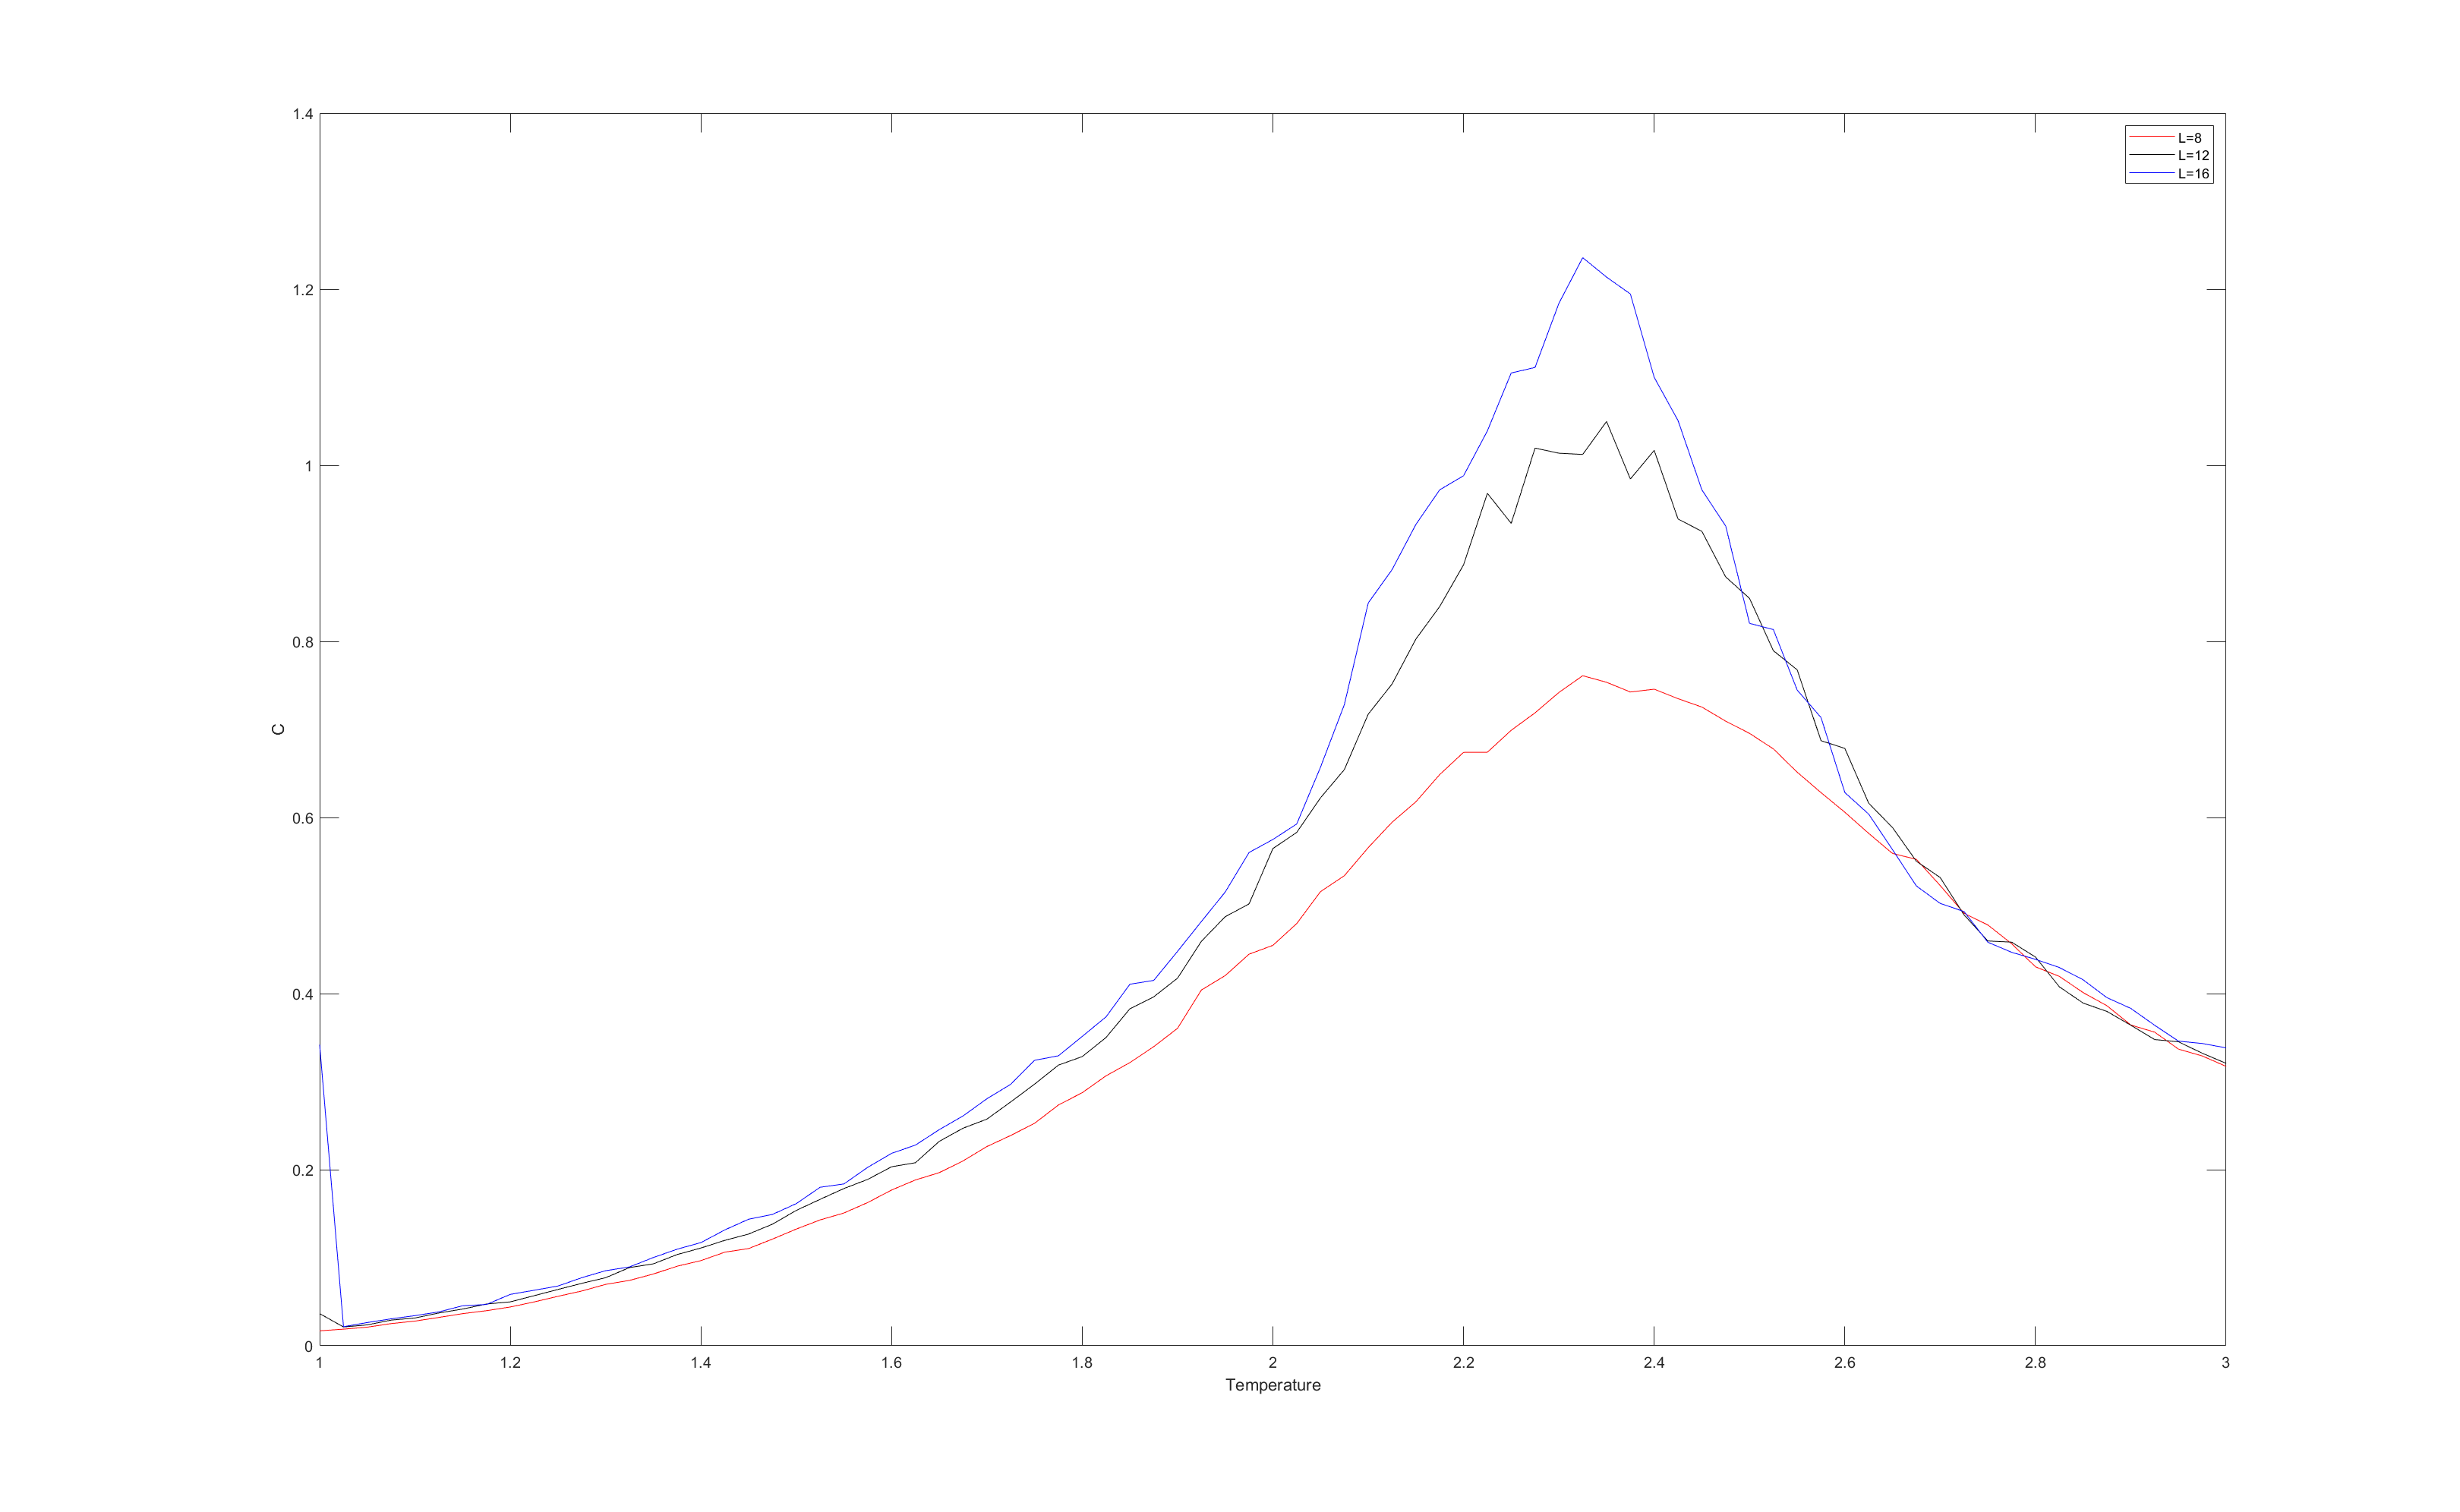
\includegraphics[width=1\textwidth,height=1\textwidth]{pictures/c.png}
    \caption{C随温度T的变化} \label{c}
\end{figure}
%以下为插入代码模板
%~\\
%\lstset{language=matlab}
%\begin{lstlisting}
%\end{lstlisting}


%%%以下为插入图片模板
%\quad \newline
%	\begin{figure}[!htbp]
%		\centering
%		\includegraphics[width=0.5\textwidth,height=0.375\textwidth]{pictures/minscale.png}
%		\caption{最小风向} \label{minsacle}
%	\end{figure}

%%%以下为插入图片模板
%\quad \newline
%	\begin{figure}[!htbp]
%		\centering
%		\includegraphics[width=0.5\textwidth,height=0.375\textwidth]{pictures/minscale.png}
%		\caption{最小风向} \label{minsacle}
%	\end{figure}

%    \begin{algorithm}
%		\caption{Title of the Algorithm}
%     	\begin{algorithmic}[1]
%			\REQUIRE some words.  % this command shows "Input"
%			\ENSURE ~\\           % this command shows "Initialized"
%			some text goes here ... \\
%			\WHILE {\emph{not converged}}
%			\STATE ... \\  % line number at left side
%			\ENDWHILE
%			\RETURN this is the lat part.  % this command shows "Output"
%		\end{algorithmic}
%	\end{algorithm}

\end{document}